%%%%%%%%%%%%%%%%%%%%%%%%%%%%%%%%%%%%%%%%%
% Beamer Presentation
% LaTeX Template
% Version 1.0 (10/11/12)
%
% This template has been downloaded from:
% http://www.LaTeXTemplates.com
%
% License:
% CC BY-NC-SA 3.0 (http://creativecommons.org/licenses/by-nc-sa/3.0/)
%
%%%%%%%%%%%%%%%%%%%%%%%%%%%%%%%%%%%%%%%%%

%----------------------------------------------------------------------------------------
%	PACKAGES AND THEMES
%----------------------------------------------------------------------------------------

\documentclass[aspectratio=169]{beamer}

\mode<presentation> {

% The Beamer class comes with a number of default slide themes
% which change the colors and layouts of slides. Below this is a list
% of all the themes, uncomment each in turn to see what they look like.

%\usetheme{default}
%\usetheme{AnnArbor}
%\usetheme{Antibes}
%\usetheme{Bergen}
%\usetheme{Berkeley}
%\usetheme{Berlin}
%\usetheme{Boadilla}
\usetheme{CambridgeUS}
%\usetheme{Copenhagen}
%\usetheme{Darmstadt}
%\usetheme{Dresden}
%\usetheme{Frankfurt}
%\usetheme{Goettingen}
%\usetheme{Hannover}
%\usetheme{Ilmenau}
%\usetheme{JuanLesPins}
%\usetheme{Luebeck}
%\usetheme{Madrid}
%\usetheme{Malmoe}
%\usetheme{Marburg}
%\usetheme{Montpellier}
%\usetheme{PaloAlto}
%\usetheme{Pittsburgh}
%\usetheme{Rochester}
%\usetheme{Singapore}
%\usetheme{Szeged}
%\usetheme{Warsaw}

% As well as themes, the Beamer class has a number of color themes
% for any slide theme. Uncomment each of these in turn to see how it
% changes the colors of your current slide theme.

%\usecolortheme{albatross}
%\usecolortheme{beaver}
%\usecolortheme{beetle}
%\usecolortheme{crane}
\usecolortheme{dolphin}
%\usecolortheme{dove}
%\usecolortheme{fly}
%\usecolortheme{lily}
%\usecolortheme{orchid}
%\usecolortheme{rose}
%\usecolortheme{seagull}
%\usecolortheme{seahorse}
%\usecolortheme{whale}
%\usecolortheme{wolverine}

%\setbeamertemplate{footline} % To remove the footer line in all slides uncomment this line
%\setbeamertemplate{footline}[page number] % To replace the footer line in all slides with a simple slide count uncomment this line
\setbeamertemplate{caption}[numbered] % numera figuras na apresentacao
%\setbeamertemplate{navigation symbols}{} % To remove the navigation symbols from the bottom of all slides uncomment this line
}

\usepackage[brazil]{babel}
\usepackage[utf8]{inputenc}
\usepackage{graphicx} % Allows including images
\usepackage{booktabs} % Allows the use of \toprule, \midrule and \bottomrule in tables
%\usepackage{enumitem} % Para criar listas "numeradas" por letras
%\usepackage{subcaption}				% Inclusão de gráficos lado a lado
%\usepackage{subfig}
\usepackage{subcaption}
\captionsetup{compatibility=false}
\usepackage{gensymb}            % Para inserir o símbolo de grau em ângulos
\usepackage[portuguese, ruled, linesnumbered]{algorithm2e} % Uso de algoritmos
\usepackage{algorithmic}
\usepackage{hyperref}
\usepackage{tabularx,ragged2e}	% Para inserir tabelas
\usepackage{multirow}			% Para mesclar células
%\usepackage[table,xcdraw]{xcolor}		% Permite adicionar cores nas linhas de tabelas
%\usepackage{color}				% Controle das cores
\usepackage{bm,amsbsy}                 % Para usar símbolos em negrito
\usepackage{amsfonts}			% Permite usar notação de conjuntos

%----------------------------------------------------------------------------------------
%	TITLE PAGE
%----------------------------------------------------------------------------------------

\title[Dissertação de Mestrado]{Introdução à Neurociência Computacional com a linguagem Python} % The short title appears at the bottom of every slide, the full title is only on the title page

\author[Weverson Nascimento]{Weverson Vieira do Nascimento} % Your name
\institute[UFPA] % Your institution as it will appear on the bottom of every slide, may be shorthand to save space
{Orientador: Prof. Dr. Antonio Pereira Junior\\
	\medskip
Universidade Federal do Pará \\ % Your institution for the title page
Programa de Pós-graduação em Engenharia Elétrica \\
\medskip
\href{mailto:weverson@ufpa.br}{\textit{weverson@ufpa.br}}
 % Your email address
}
\date{\today} % Date, can be changed to a custom date

\subject{Apresentação de Dissertação de Mestrado com título "Introdução à Neurociência Computacional com a linguagem Python", apresentado para obtenção do grau de Mestre em Engenharia Elétrica pela Universidade Federal do Pará. Área de concentração: Engenharias.}
% This is only inserted into the PDF information catalog. Can be left out. 
  
\keywords{Neurociência computacional. Python. Conexões neuronais. Inteligência artificial.}

\pgfdeclareimage[height=0.9cm]{ufpa-logo}{modelo-ufpa/logo-eps-converted-to.pdf}
\logo{\pgfuseimage{ufpa-logo}\hspace*{0.3cm}}


% Delete this, if you do not want the table of contents to pop up at
% the beginning of each subsection:
%\AtBeginSection[]
%{
%  \begin{frame}<beamer>{Agenda}
%  	\tableofcontents[currentsection]
%  \end{frame}
%}


% If you wish to uncover everything in a step-wise fashion, uncomment
% the following command: 

%\beamerdefaultoverlayspecification{<+->}

% To include notes
\setbeameroption{show notes on second screen}


\begin{document}
	\begin{frame}
		\titlepage % Print the title page as the first slide
	\end{frame}
	
	\begin{frame}
		\frametitle{Agenda} % Table of contents slide, comment this block out to remove it
		\tableofcontents % Throughout your presentation, if you choose to use \section{} and \subsection{} commands, these will automatically be printed on this slide as an overview of your presentation
		% You might wish to add the option [pausesections]
	\end{frame}

	\section{Introdução} 
\begin{frame}\frametitle{Introdução}
	Elaborar um roteiro para execução de um curso introdutório em neurociências computacionais usando linguagens de programação livres
\end{frame}

	\section{Base teórica}
\subsection*{Neurobiologia básica}
\begin{frame}
	\begin{columns}[t]
		\column{5cm}
			\begin{figure}[tb]
				\centering
				\caption{Neurônio}
				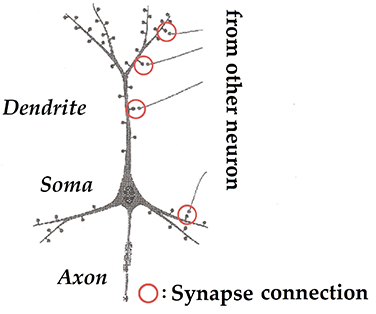
\includegraphics[width=0.55\linewidth]{figs/neuronio}
				\label{fig:neuronio}
				%		\fonte{Adaptado de \cite{lopez-ruiz_simulation_2016}}
				%TODO: trocar figura
			\end{figure}
		\column{5cm}
			\begin{itemize}
				\item Composto pelo núcleo (soma), dendritos, axônio e terminais axonais;
				\item contém íons e moléculas, positivas ou negativas.
				\note{Teste de nota}
			\end{itemize}
	\end{columns}
\end{frame}

\begin{frame}
	\begin{columns}[t]
		\column{5cm}
			\begin{figure}[tb]
				\centering
				\caption{Membrana do neurônio}
				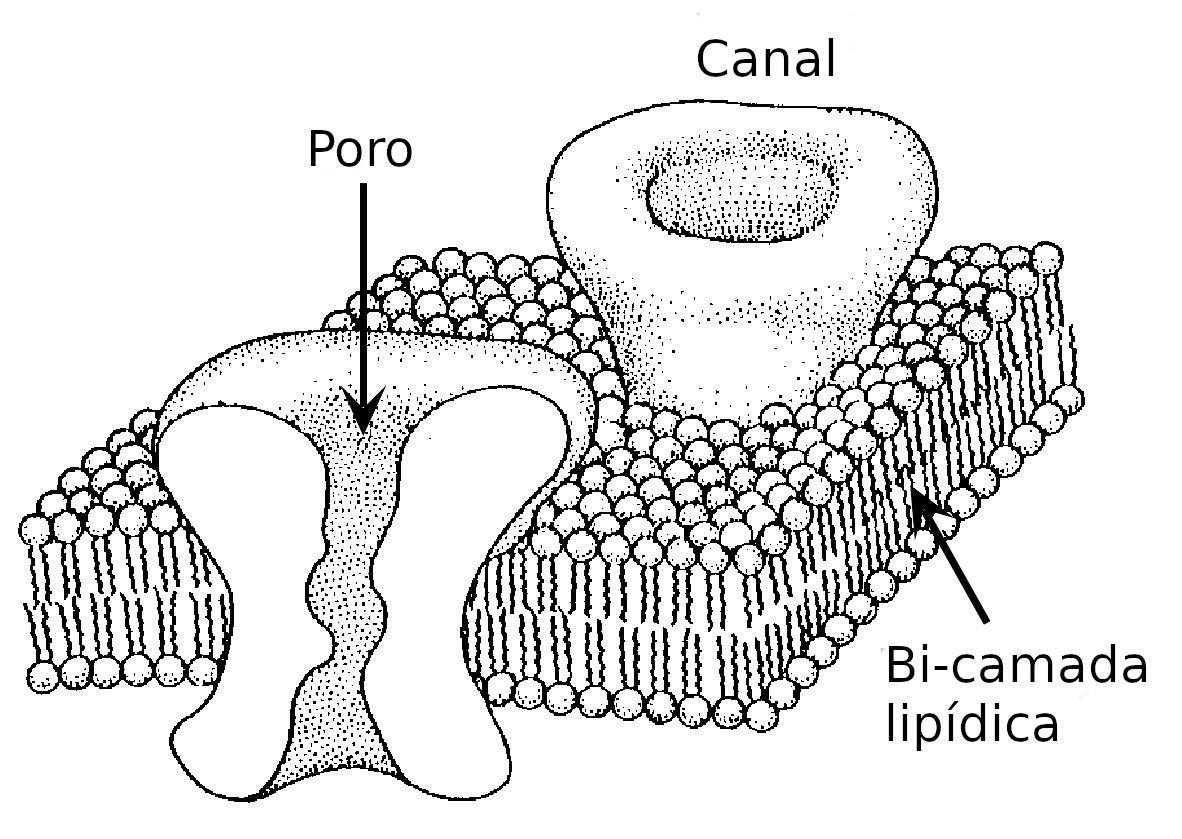
\includegraphics[width=0.55\linewidth]{figs/membrana_neuronio}
				\label{fig:membrananeuronio}
%				\fonte{adaptado de \cite{hille_ionic_1992}}
			\end{figure}
		\column{5cm}
			\begin{itemize}
				\item O interior da célula, geralmente, possui mais cargas negativas;
				\item o potencial de membrana fica a maior parte do tempo negativo;
				\note{potencial de membrana: diferença entre o potencial interno e o externo da célula neuronal}
				\item o fluxo de íons através dos poros de canais iônicos altera o potencial de membrana.
			\end{itemize}
	\end{columns}
\end{frame}

\begin{frame}
	\begin{columns}[t]
		\column{5cm}
			\begin{figure}[tb!]
				\centering
				\caption{Canais iônicos de potássio}
				\label{fig:canaisions}
				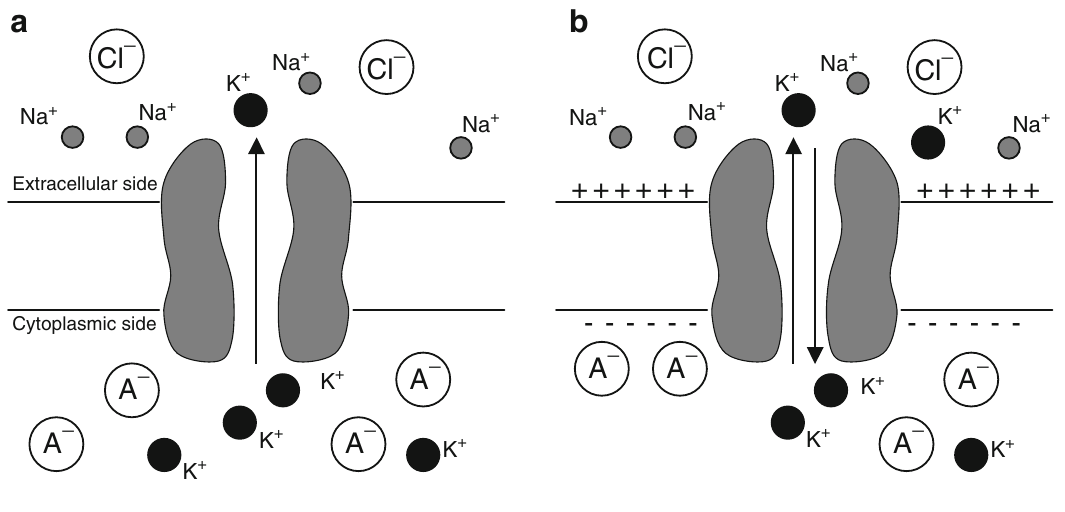
\includegraphics[width=0.7\linewidth]{figs/canais_ions}
%				\fonte{Adaptado de \cite{ermentrout_mathematical_2010}}
			\end{figure}
		\column{5cm}
			\begin{itemize}
				\item Canais iônicos permitem a movimentação de íons através deles;
				\item podem ser sem portão, que estão sempre abertos, ou com portão, que podem abrir ou fechar;
				\item quando não há fluxo de íons e o potencial de membrana não se altera ele é chamado de potencial de repouso.
				\note{valor típico do potencial de repouso: $-70\ mv$}
			\end{itemize}
	\end{columns}
\end{frame}

\begin{frame}
	\begin{columns}[t]
		\column{5cm}
			\begin{itemize}
				\item Despolarização: quando íons positivos entram na célula, deixando o potencial de membrana mais positivo;
				\item Hiperpolarização: quando íons negativos entram na célula, ou positivos saem, deixando o potencial de membrana mais negativo;
				\item o potencial de membrana é dado na forma de uma equação diferencial.
			\end{itemize}
		\column{5cm}
			\[
				\frac{\mathrm{d}V_m}{\mathrm{d}t}=G_l(E_l-V_m)/C_m
			\]
			\begin{itemize}
				\item $V_m$: potencial de membrana
				\item $C_m$: capacitância da membrana
				\item $E_l$: potencial de vazamento
				\item $G_l$: condutância de vazamento
			\end{itemize}
	\end{columns}
\end{frame}

\subsection*{Equações diferenciais ordinárias}
\begin{frame}
	\begin{columns}[t]
		\column{5cm}
			\begin{figure}
				\centering
				\caption{Soluções da equação $y'=y-t$ para vários $c$}
				\label{fig:solucao}
				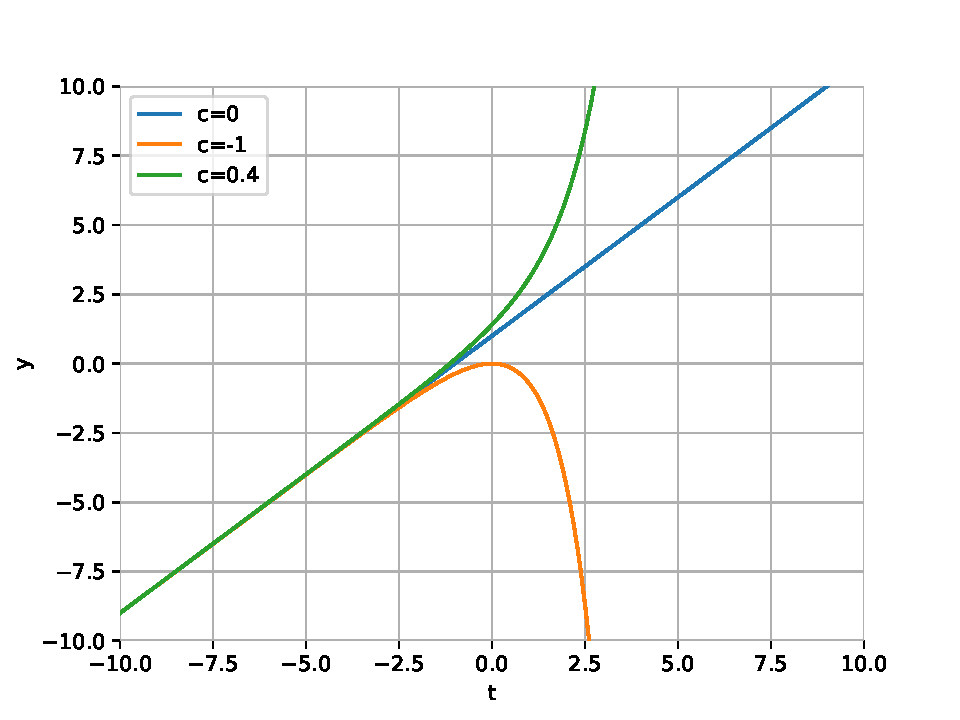
\includegraphics[width=0.7\linewidth]{figs/solucao}
%				\fonte{O autor (\the\year)}
			\end{figure}
			\note{solução: $y(t) = t + 1 + ce^t$}
		\column{5cm}
			\[
				\frac{\mathrm{d}y(t)}{\mathrm{d}t}=f(y(t))
			\]
			\begin{itemize}
				\item Equações diferenciais: descrevem sistemas dinâmicos;
				\item possuem como solução uma família de equações;
				\item podem ser resolvidas de maneira analítica ou numérica.
			\end{itemize}
	\end{columns}
\end{frame}

\begin{frame}
	\begin{columns}[t]
		\column{5cm}
			\begin{figure}[tb]
				\centering
				\caption{Método de Euler}
				\label{fig:euler}
				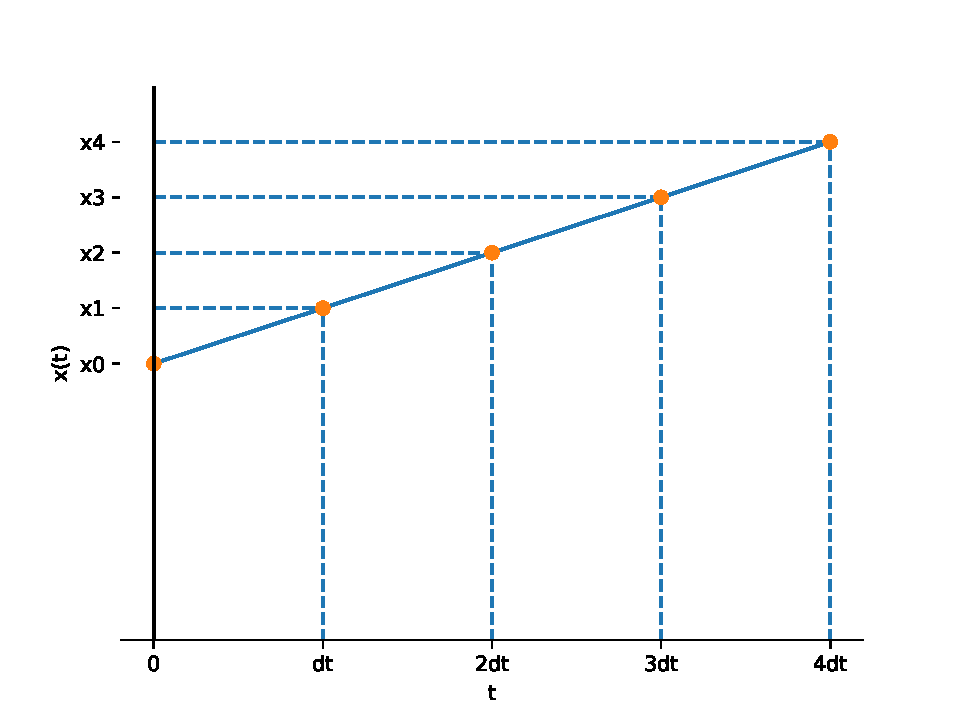
\includegraphics[width=0.7\linewidth]{figs/euler}
%				\fonte{O autor (\the\year)}
			\end{figure}
		\column{5cm}
		\begin{itemize}
			\item Método de Euler: soluciona numericamente equações diferenciais;
			\item considera um valor inicial ($X_0$) e intervalos discretos fixos ($\Delta t$);
			\item calcula o valor seguinte ($x_{n+1}$) a partir do atual ($x_n$);
			\item o algoritmo para utilizá-lo é implementado em Python.
			\note{Algoritmo: sequência de instruções para executar uma determinada tarefa}
		\end{itemize}
		\[
			x_{n+1}=x_n+f(x_n,t_n)\Delta t
		\]
	\end{columns}
\end{frame}

	\section{Modelos de neurônio de disparo}
\subsection{Leaky integrate-and-fire}
\begin{frame}{Circuito equivalente da membrana neuronal}
	\begin{columns}[t]
		\column{5cm}
			\begin{figure}[htb!]
				\centering
				\caption{Circuito equivalente da membrana}
				\label{fig:circuitomembrana}
				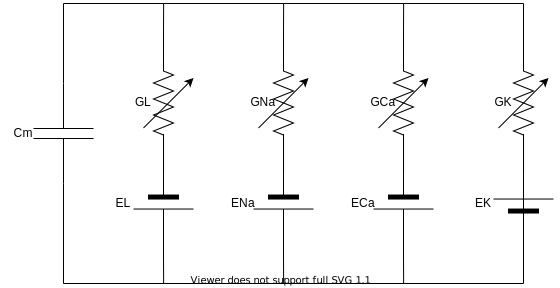
\includegraphics[width=\linewidth]{figs/circuito_membrana}
%				\fonte{O autor (\the\year)}
			\end{figure}
		\column{5cm}
			\begin{itemize}
				\item O capacitor está associado à capacitância de membrana;
				\item $G_L$ e $E_L$ referem-se aos elementos de vazamento;
				\item os demais são referentes aos canais iônicos dependentes de tensão.
				\note{na: sódio}
				\note{ca: cálcio}
				\note{k: potássio}
			\end{itemize}
	\end{columns}
	\vfill
	\[
		c_m\frac{\mathrm{d}V_m}{\mathrm{d}t}=G_{Na}(E_{Na}-V_m)+G_{Ca}(E_{Ca}-Vm)+G_K(E_K-V_m)+G_L(E_L-V_m)
	\]
\end{frame}

\begin{frame}{Modelo \textit{Leaky integrate-and-fire} (LIF)}
	\begin{columns}[t]
		\column{5cm}
			\begin{figure}[htb!]
				\centering
				\caption{Circuito equivalente do modelo LIF}
				\label{fig:circuitolif}
				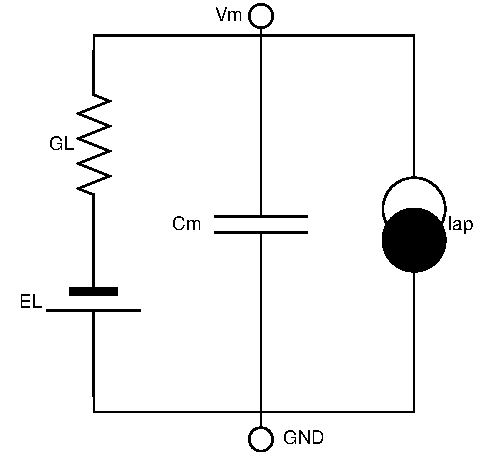
\includegraphics[width=0.5\linewidth]{figs/circuito_lif}
%				\fonte{O autor (\the\year)}
				%TODO: trocar GND
			\end{figure}
		\column{5cm}
			\begin{itemize}
				\item inclui uma corrente ($I_{ap}$) que é acumulada (integrada);
				\item contém uma condição que força o disparo (\textit{fire}) do potencial de ação no valor limite ($V_{th}$);
				\item no disparo, o potencial de membrana é atualizado para um valor de \textit{reset} ($V_{reset}$).
				\note{o modelo não representa a hiperpolarização que ocorre após o disparo, por isso o reset é acrescentado}
			\end{itemize}
	\end{columns}
	\vfill
	\[
		c_m\frac{dV_m}{dt} = G_L(E_L-V_m)+I_{ap}; \text{ se } V_m > V_{th} \text{ então } V_m\mapsto V_{reset}
	\]
\end{frame}

\begin{frame}{Modelo \textit{Leaky integrate-and-fire} (LIF)}
	\begin{figure}
		\centering
		\caption{Exemplo da simulação com o modelo LIF}
		\label{fig:lif}
		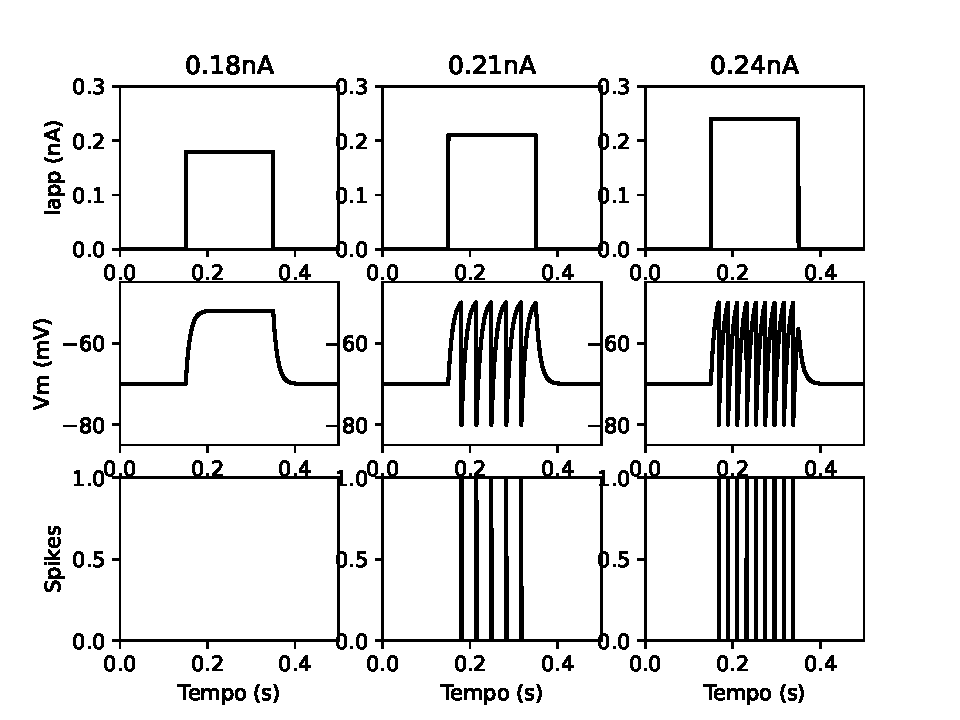
\includegraphics[width=0.5\linewidth]{figs/lif}
%		\fonte{O autor (\the\year)}
		%TODO: regerar
	\end{figure}
\end{frame}

\begin{frame}{Período refratário}
	\begin{columns}[t]
		\column{5cm}
			\begin{figure}
				\centering
				\caption{Simulação do modelo LIF com período refratário}
				\label{fig:lifrefratario}
				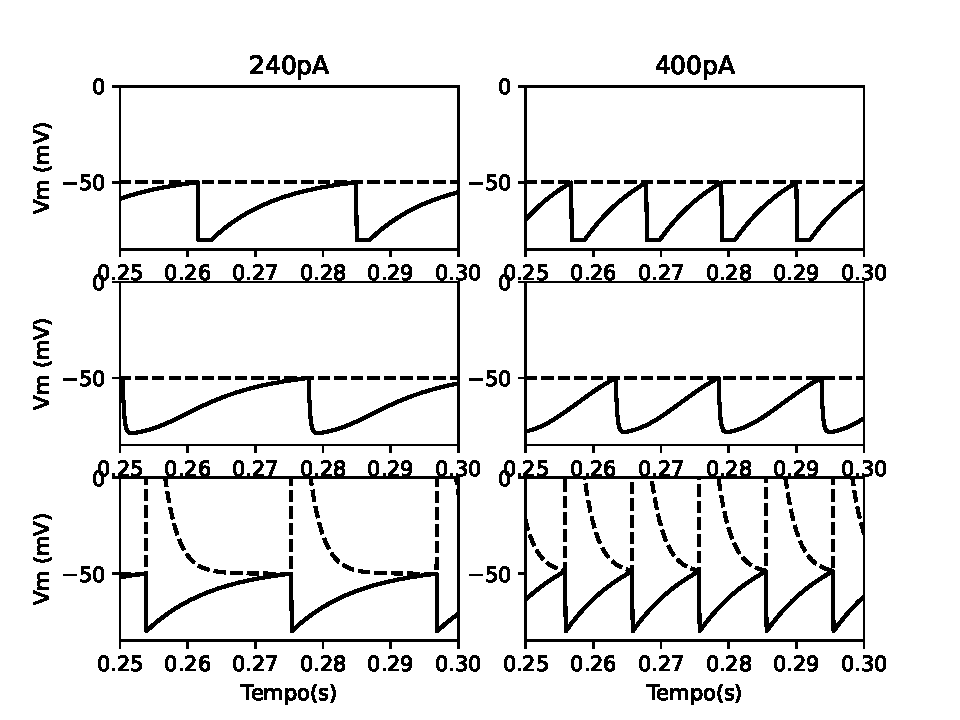
\includegraphics[width=\linewidth]{figs/lif_refratario}
%				\fonte{O autor (\the\year)}
				%TODO: regerar
			\end{figure}
		\column{5cm}
		\begin{itemize}
			\item intervalo de tempo que o neurônio não produz um novo disparo;
			\item não é presente no modelo LIF, por isso é acrescentado como extensão;
			\item métodos existentes para simular incluem o grampeamento de tensão, a condutância refratária e o incremento do limiar.
			\note{grampeamento de tensão: fixa o potencial de membrana no valor de reset}
			\note{condutância refratária: acrescenta uma condutância elevada, geralmente uma corrente hiperpolarizante de potássio, fazendo com que o potencial de membrana cresça em um ritmo mais lento}
			\note{incremento do limiar: aumenta o valor do limiar após cada potencial de ação}
		\end{itemize}
	\end{columns}
\end{frame}

\begin{frame}{Adaptação da taxa de disparos}
	\begin{columns}[t]
		\column{5cm}
			\begin{figure}
				\centering
				\caption{Adaptação da taxa de disparo no neurônio LIF}
				\label{fig:lifatd}
				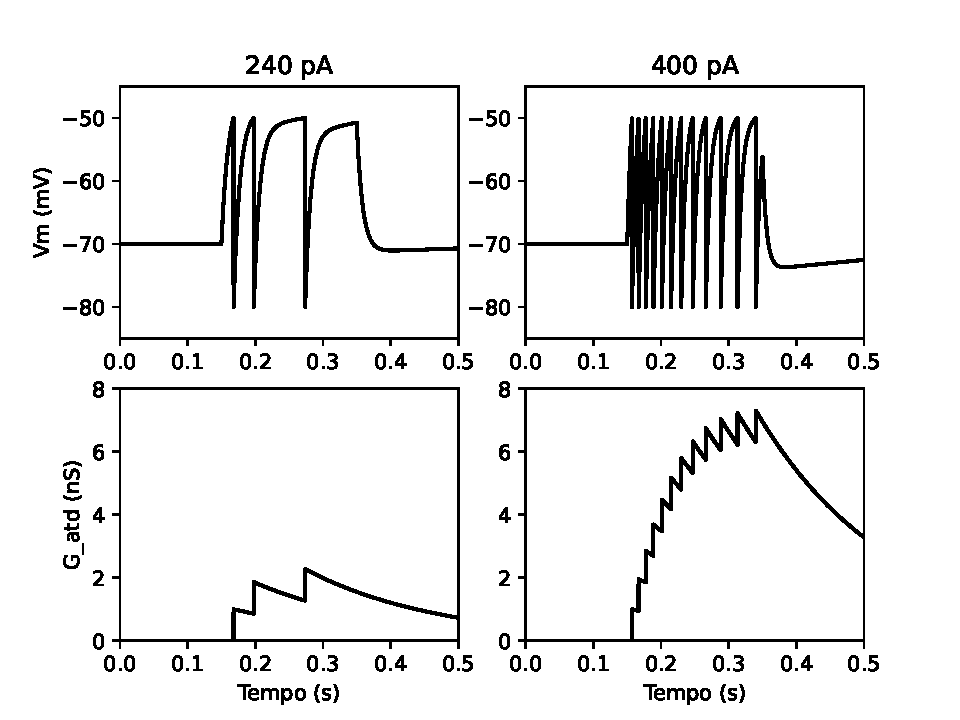
\includegraphics[width=\linewidth]{figs/lif_atd}
%				\fonte{O autor (\the\year)}
				%TODO: regerar
			\end{figure}
		\column{5cm}
		\begin{itemize}
			\item Diminuição da taxa de disparos logo após o primeiro; 
			\item é implementado de maneira semelhante ao método da condutância refratária;
			\item difere pelo valor do incremento de condutância, que é menor, e a escala de tempo, que é maior.
			\note{Uma fácil percepção da consequência da adaptação da taxa de disparo é a diferença de percepção de cheiros intensos ao longo do tempo, como quando uma pessoa entra com um perfume forte em um elevador}
			\note{o incremento menor não impede o disparo de novos potenciais, só diminui a taxa}
			\note{a escala de tempo maior permite o acúmulo das condutâncias ao longo da sequência de disparos}
		\end{itemize}
	\end{columns}
\end{frame}

\begin{frame}{Modelo \textit{Exponential leaky integrate-and-fire} (ELIF)}
	\begin{columns}[t]
		\column{5cm}
			\begin{figure}[tb]
				\centering
				\caption{Comparação dos modelos LIF e ELIF}
				\label{fig:elif}
				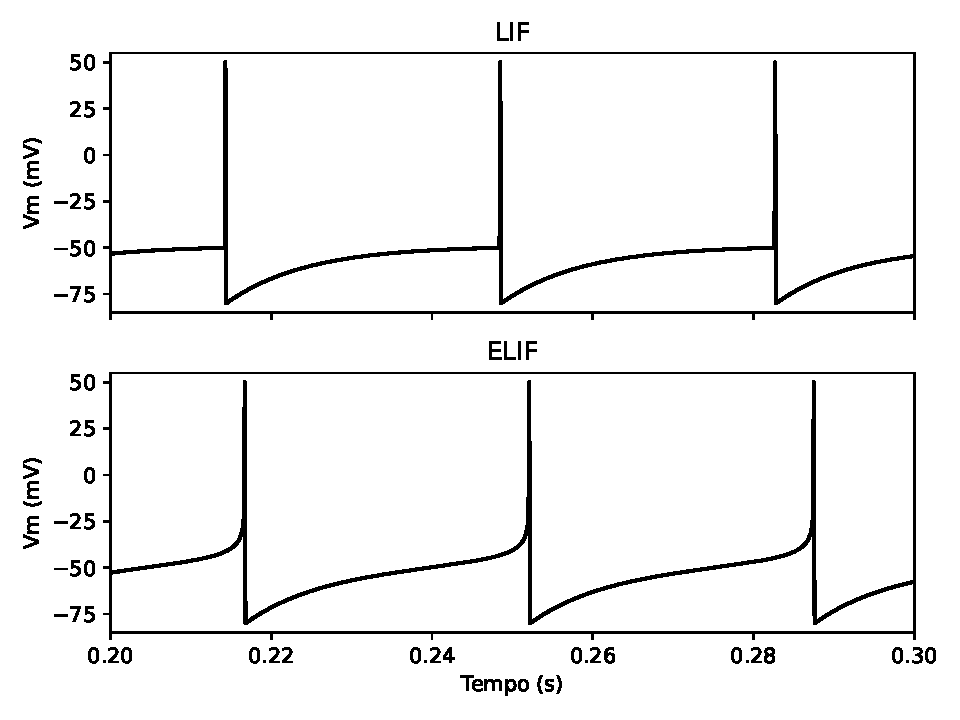
\includegraphics[width=0.8\linewidth]{figs/elif}
%				\fonte{O autor (\the\year)}
				%TODO: regerar
			\end{figure}
			\[
				\text{se } V_m > V_{max} \text{ então } V_m\mapsto V_{reset}
			\]
		\column{5cm}
		\begin{itemize}
			\item Incorpora um termo adicional para a geração do potencial de ação;
			\item acrescenta uma corrente despolarizante que eleva quase instantaneamente o valor do potencial de membrana;
			\item o crescimento tende ao infinito, mas é definido um limite nas simulações.
			\note{o computador tem problemas com valores infinitos, por isso o limite}
		\end{itemize}
	\end{columns}
	\vfill
	\[
	c_m\frac{dV_m}{dt} = G_L(E_L-V_m) + G_L\Delta_{th}\exp\Big(\frac{V_m-V_{th}}{\Delta_{th}}\Big) + I_{ap}
	\]
\end{frame}

\begin{frame}{Modelo \textit{Adaptative exponential leaky integrate-and-fire} (AELIF)}
	\begin{columns}[t]
		\column{5cm}
			\begin{figure}[tb]
				\centering
				\caption{Resposta do modelo AELIF}
				\label{fig:adexrs}
				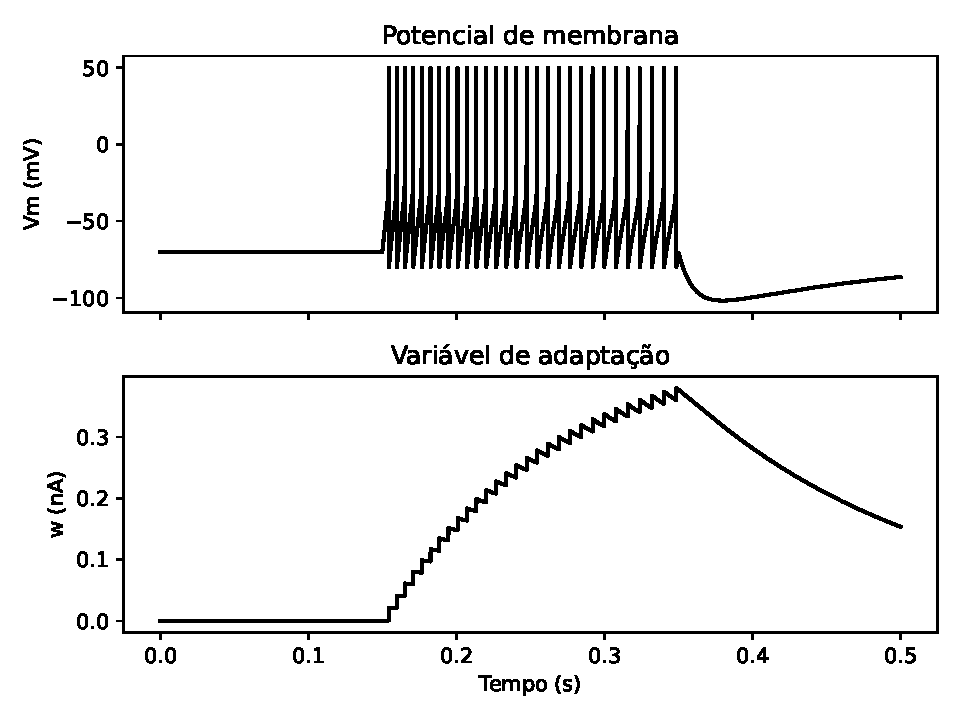
\includegraphics[width=0.8\linewidth]{figs/aelif}
%				\fonte{O autor (\the\year)}
				%TODO: regerar
			\end{figure}
			\note{Resposta do modelo AELIF para um pulso de corrente de 1 $nA$}
		\column{5cm}
		\begin{itemize}
			\item Adiciona uma corrente adaptativa hiperpolarizante;
			\item modelo de duas equações, para o potencial de membrana e a variável de adaptação ($w$).
			\note{a: parâmetro de agrupamento}
			\note{b: parâmetro de adaptação (incremento de corrente após o disparo)}
			\note{a curva de adaptação é semelhante à condutância adaptativa e condutância refratária}
		\end{itemize}
		\[
			\text{se } V_m > V_{max} \text{: } V_m\mapsto V_{reset} \text{ e } w\mapsto w + b
		\]
	\end{columns}
	\vfill
	\[
	c_m\frac{dV_m}{dt} = G_L(E_L-V_m) + G_L\Delta_{th}\exp\Big(\frac{V_m-V_{th}}{\Delta_{th}}\Big) - w + I_{ap}
	\]\[
	\tau_w\frac{dw}{dt}=a(V_m-E_L)-w
	\]
\end{frame}

\subsection{Izhikevich}

\subsection{Hodgkin-Huxley}

	\section{Conexões entre neurônios}
\subsection{Sinapses}
\begin{frame}{Sinapses}
	\begin{columns}[t]
		\column{5cm}
			\begin{figure}[tb]
				\centering
				\caption{Esquema simplificado de uma sinapse química}
				\label{fig:sinapses}
				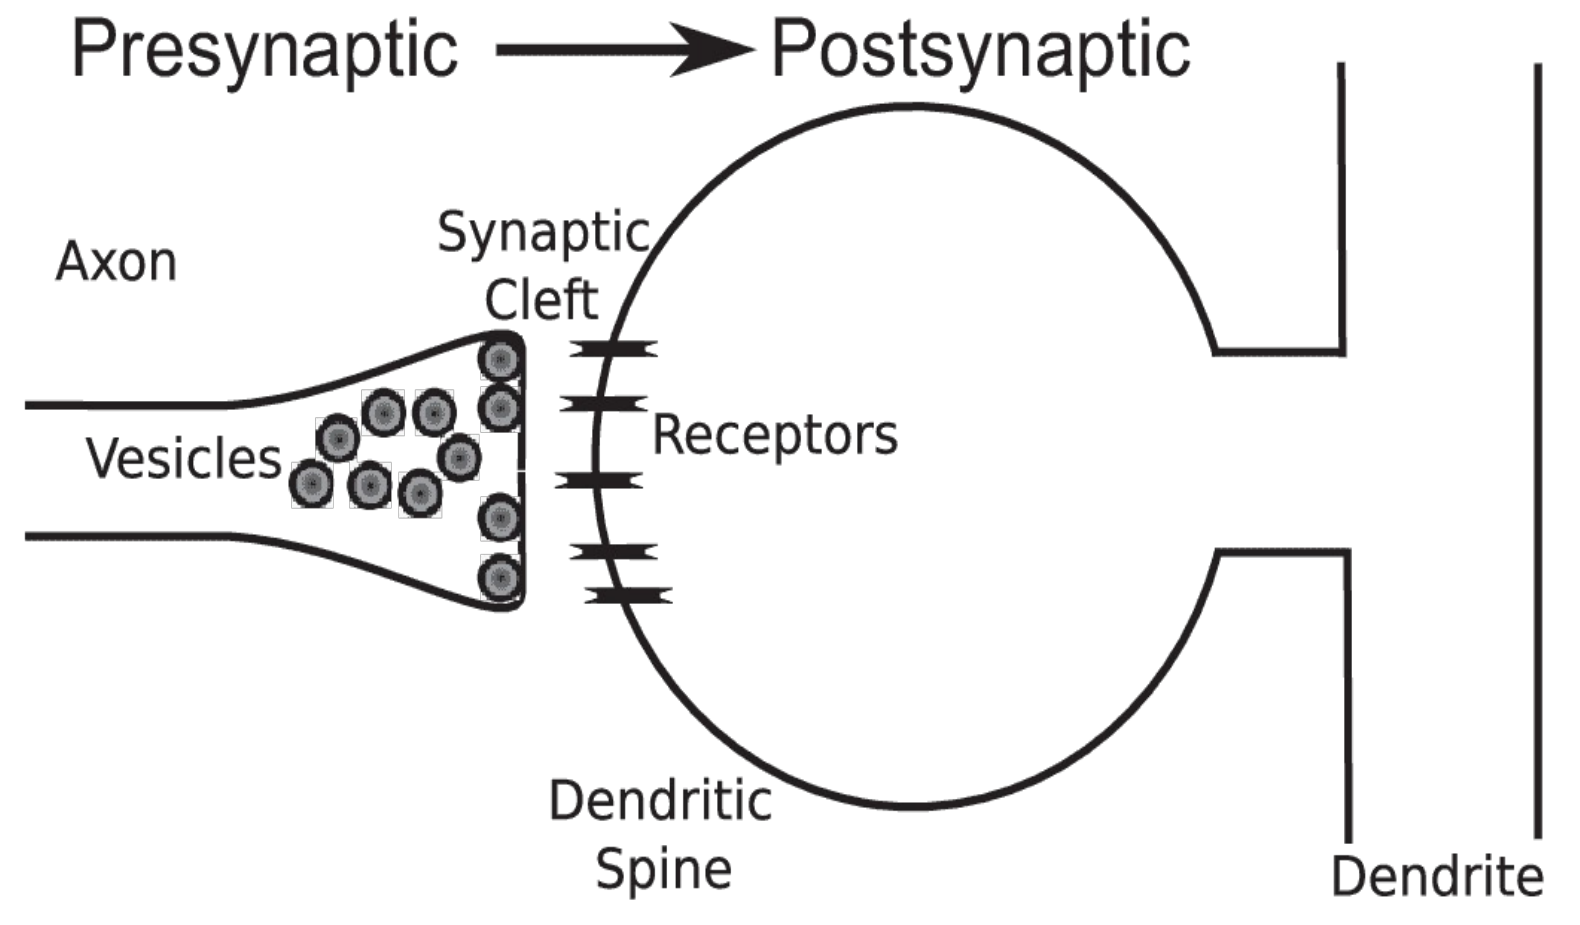
\includegraphics[width=0.9\linewidth]{figs/sinapses}\\
%				\fonte{\cite{miller_introductory_2018}}
				%TODO: trocar figura
			\end{figure}
		\column{5cm}
			\begin{itemize}
				\item Conexão entre dois neurônios;
				\item elétricas: se dão a partir de uma junção entre duas células;
				\item químicas: conectadas por um espaço entre as células por meio de neurotransmissores.
				\item excitatórias: despolarizam a membrana; inibitórias: hiperpolarizam
				\note{glutamato: excita a célula}
				\note{gaba: normalmente inibe}
			\end{itemize}
	\end{columns}
\end{frame}

\begin{frame}{Sinapses}
	\begin{columns}[t]
		\column{5cm}
			\begin{figure}[tb]
				\centering
				\caption{Condutância sináptica em resposta aos potenciais de ação da célula pré-sináptica}
				\label{fig:respostasinaptica}
				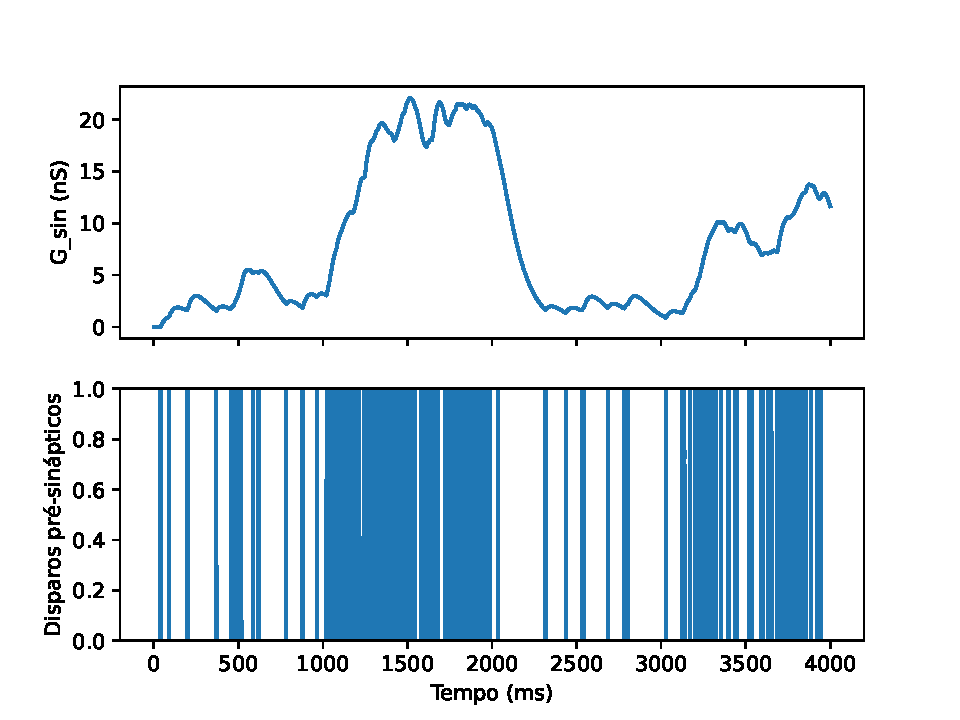
\includegraphics[width=0.9\linewidth]{figs/resposta_sinaptica}
%				\fonte{O autor (\the\year)}
				%TODO: regerar
			\end{figure}
		\column{5cm}
			\[
				\frac{dG_{sin}(t)}{dt}=\frac{-G_{sin}(t)}{\tau_{sin}}
			\]\[
				G_{sin}(t)\mapsto G_{sin}(t)+\Delta G
			\]
			\begin{itemize}
				\item $G_{sin}(t)$: condutância sináptica
				\item $\tau_{sin}$: constante de tempo
				\item $\Delta G$: incremento de condutância
			\end{itemize}
	\end{columns}
\end{frame}

\begin{frame}{Sinapses dinâmicas}
	\begin{columns}[t]
		\column{5cm}
			\begin{figure}[tb]
				\centering
				\caption{Depressão e facilitação sináptica}
				\label{fig:plasticidadecurtaduracao}
				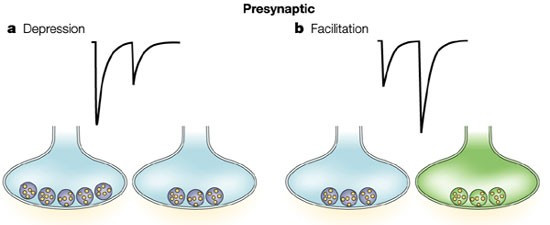
\includegraphics[width=0.9\linewidth]{figs/plasticidade_curta_duracao}
%				\fonte{Adaptado de \cite{blitz_short-term_2004}}
				%TODO: trocar figura
			\end{figure}
		\column{5cm}
			\begin{itemize}
				\item Depressão de curta duração: redução temporária na força sináptica;
				\item Facilitação de curta duração: incremento temporário na força sináptica
			\end{itemize}
	\end{columns}
	\[
		\begin{aligned}
			\frac{dD}{dt}&=\frac{1-D}{\tau_D} &\qquad &D\mapsto D-p_0FD\\
			\frac{dF}{dt}&=\frac{1-F}{\tau_F} &\qquad &F\mapsto F+f_{fat}(F_{max}-F)
		\end{aligned}
		\qquad\qquad \Delta G=G_{max}p_0FD
	\]
\end{frame}

\subsection{Multi-estabilidade}
\begin{frame}{Multi-estabilidade}
	\begin{columns}[t]
		\column{5cm}
			\begin{figure}[tb]
				\centering
				\caption{Comportamento variado do modelo de Hodgkin-Huxley}
				\label{fig:hhdinamico}
				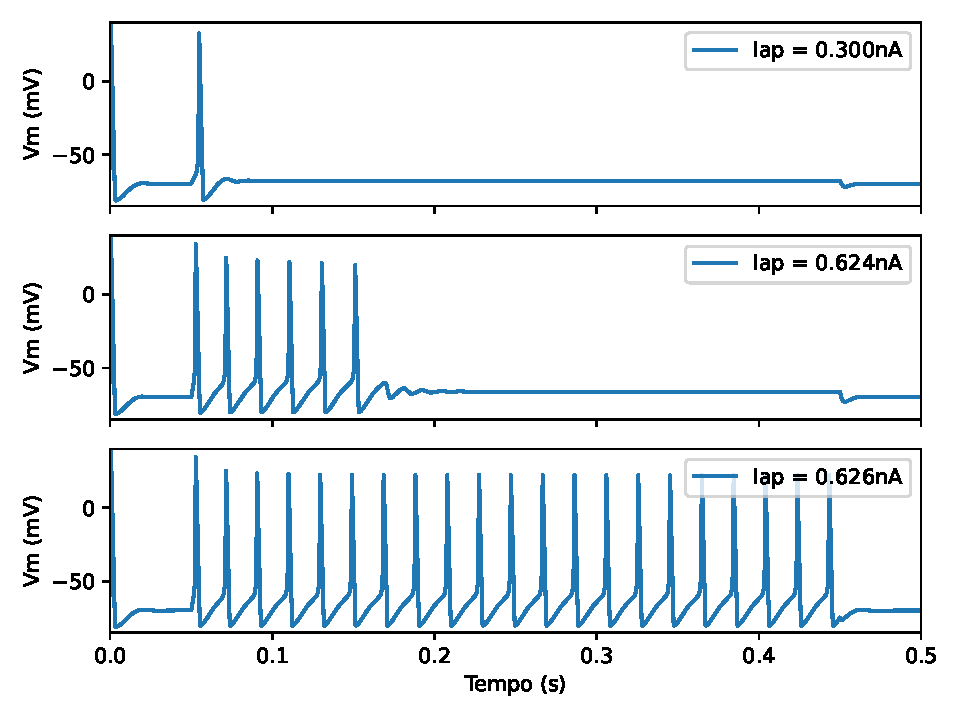
\includegraphics[width=0.9\linewidth]{figs/hh_dinamico}
%				\fonte{O autor (\the\year)}
				%TODO: regerar
			\end{figure}
		\column{5cm}
			\begin{itemize}
				\item Capacidade dos neurônios de manterem múltiplos estados mesmo com a mesma entrada;
				\item Hodgkin-Huxley, por exemplo, pode alternar entre oscilações e ressonância
			\end{itemize}
	\end{columns}
\end{frame}

\begin{frame}{Bi-estabilidade}
	\begin{columns}[t]
		\column{5cm}
			\begin{figure}[tb]
				\centering
				\caption{Cubo de Necker}
				\label{fig:cubonecker}
				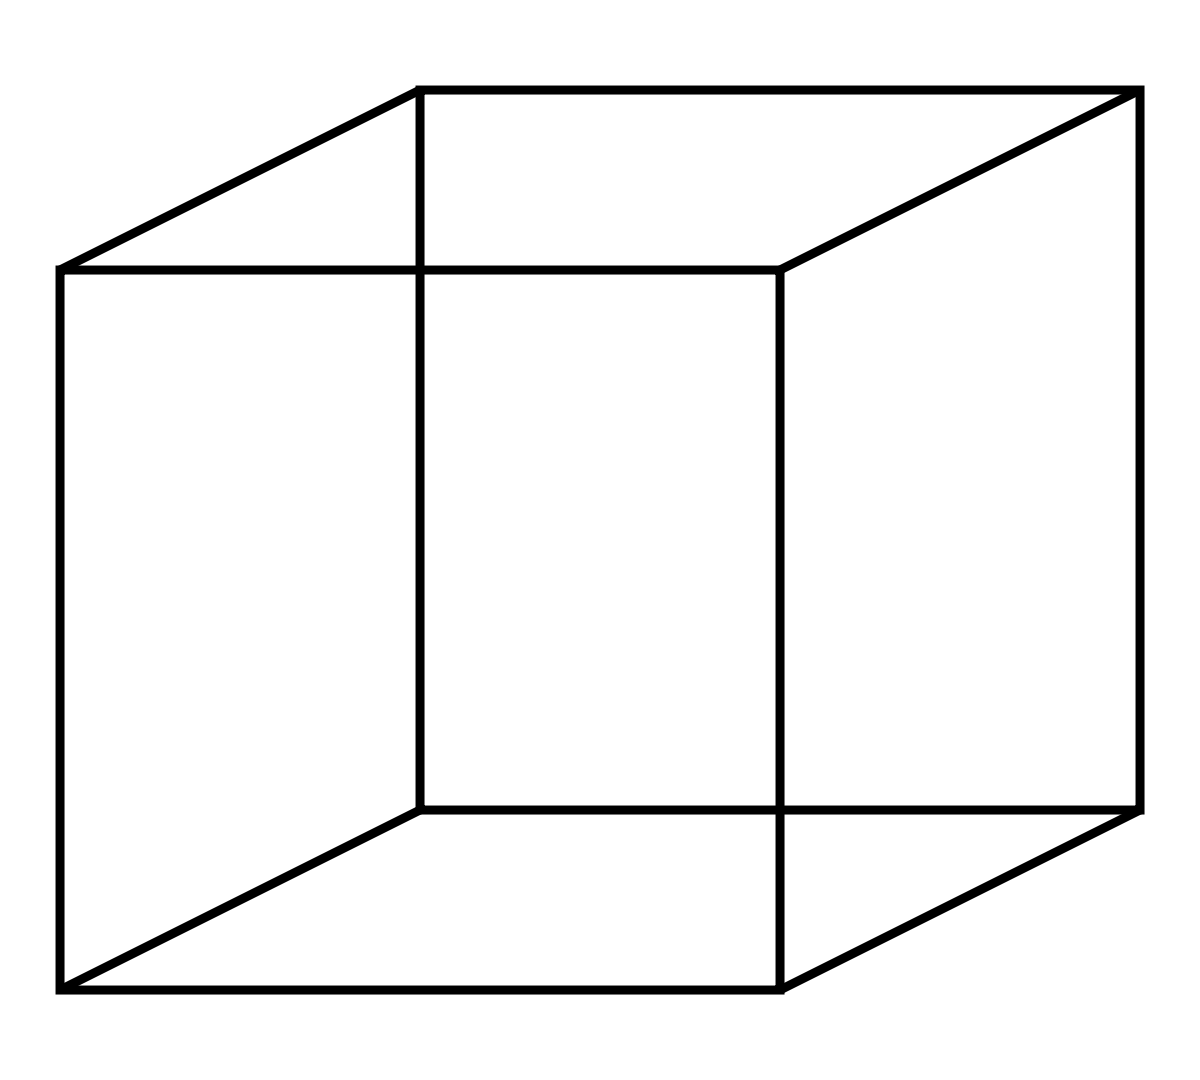
\includegraphics[width=0.7\textwidth]{figs/cubo_necker}
%				\fonte{Domínio público}
			\end{figure}
		\column{5cm}
			\begin{itemize}
				\item Forma mais simples de multi-estabilidade;
				\item dois estados de atividade podem ocorrer;
				\item causa a rivalidade perceptual: estímulos únicos podem ser percebidos de mais de uma maneira
			\end{itemize}
	\end{columns}
\end{frame}


\begin{frame}{Unidades de decisão}
	\begin{columns}[t]
		\column{5cm}
			\begin{figure}[tb]
				\centering
				\caption{Unidades de decisão com feedback recorrente e interconexão}
				\label{fig:unidadesdecisao}
				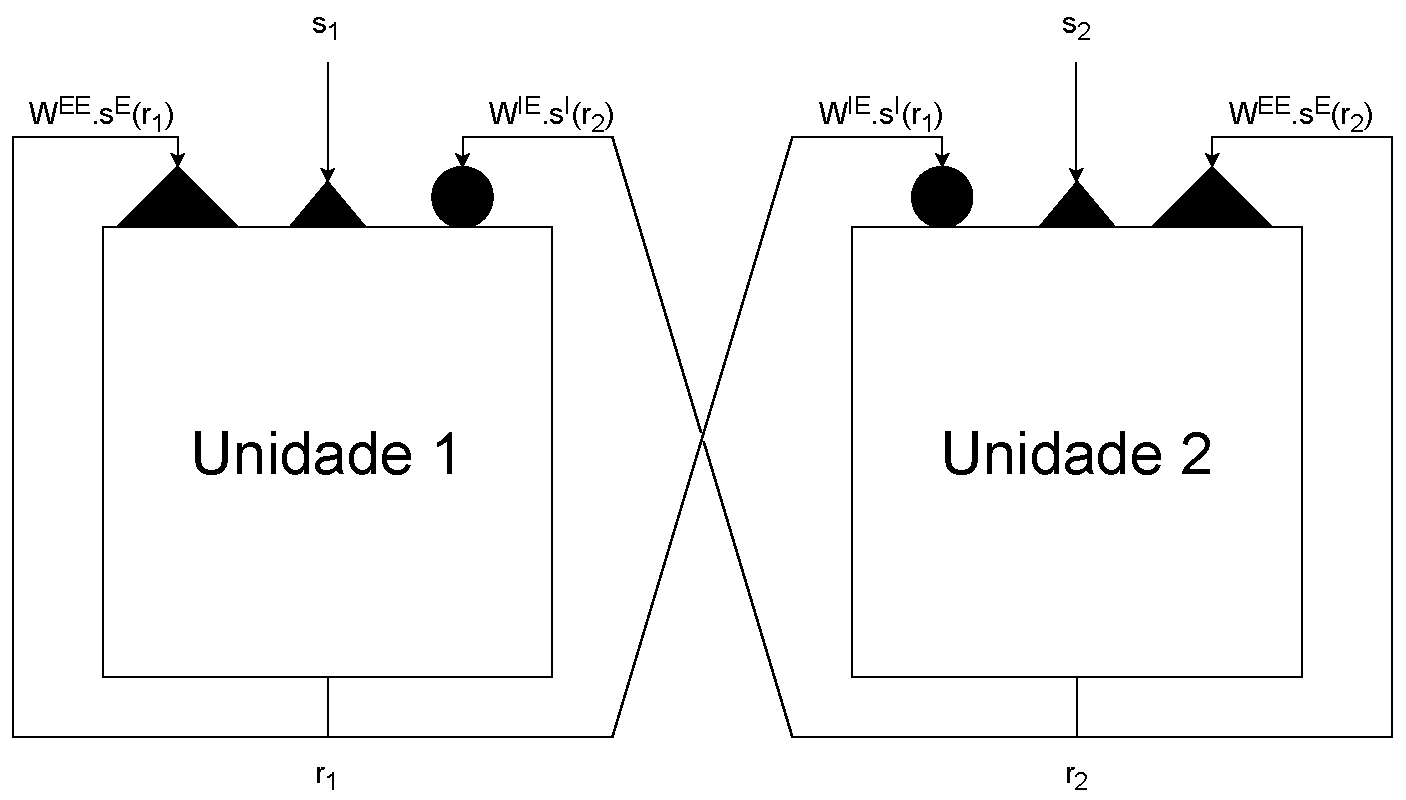
\includegraphics[width=\linewidth]{figs/unidades_decisao}
%				\fonte{O autor (\the\year)}
			\end{figure}
		\column{5cm}
			\begin{itemize}
				\item grupo de neurônios onde é considerada a atividade média deles;
				\note{as entradas diferem por ruído}
				\item unidades podem ter interconexão, com uma inibindo a outra;
				\item podem conectar a si mesmas (\textit{feedback} recorrente).
				\note{o ruído, tanto na entrada quanto dentro da unidade, pode induzir às transições entre estados}
			\end{itemize}
	\end{columns}
\end{frame}

\begin{frame}{Circuito gerador de padrão central}
	\begin{columns}[t]
		\column{5cm}
			\begin{figure}[tb]
				\centering
				\caption{Gerador de padrão central de duas unidades}
				\label{fig:cpg}
				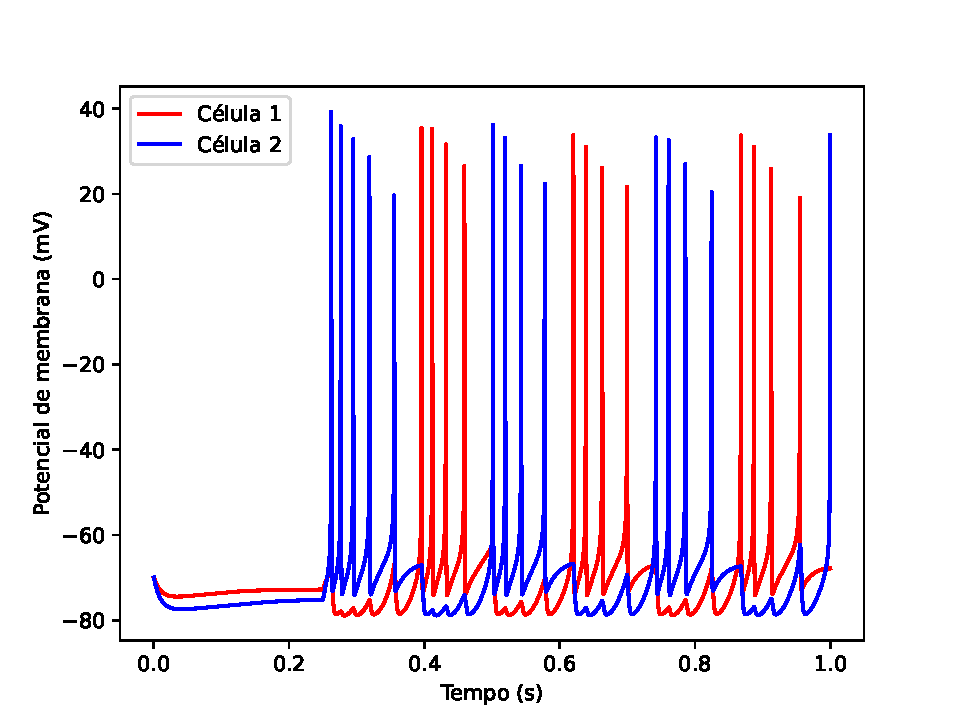
\includegraphics[width=\linewidth]{figs/cpg}
%				\fonte{O autor (\the\year)}
			\end{figure}
		\column{5cm}
			\begin{itemize}
				\item reproduzem padrões rítmicos de atividade neuronal sem receber entradas rítmicas;
				\item a ativação de uma célula inibe a outra;
				\note{correlato com a locomoção: movimento das duas pernas}
				\item muito aplicados em circuitos associados à locomoção de robôs articulados.
			\end{itemize}
	\end{columns}
\end{frame}

\begin{frame}{Circuitos de tomada de decisão}
	\begin{columns}[t]
		\column{5cm}
			\begin{figure}[tb]
				\centering
				\caption{Circuito de tomada de decisão}
				\label{fig:tomadadecisao}
				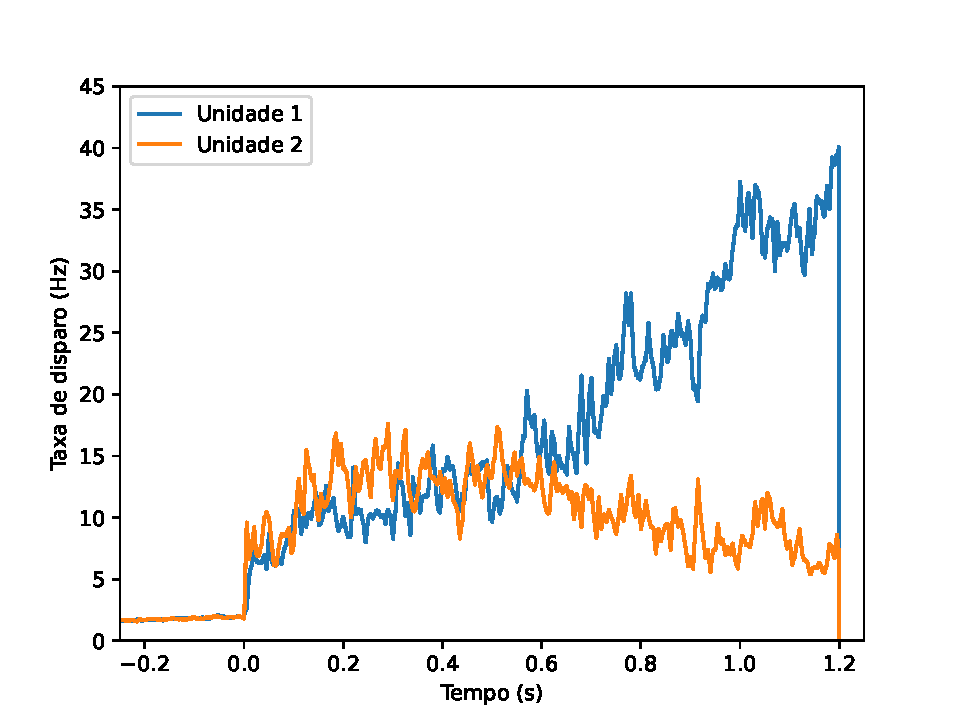
\includegraphics[width=\linewidth]{figs/tomada_decisao}
%				\fonte{O autor (\the\year)}
			\end{figure}
		\column{5cm}
			\begin{itemize}
				\item Acumulam informações sensoriais ao longo do tempo até uma decisão ser tomada;
				\item cada unidade acumula evidências do estímulo ao longo do tempo;
				\item a primeira unidade a atingir um limiar é considerada a vencedora.
				\note{limiar de 40 Hz}
			\end{itemize}
	\end{columns}
\end{frame}

\subsection{Modelos de taxa de disparo}
\begin{frame}{Modelo de Wilson-Cowan}
	\begin{figure}
		\centering
		\caption{Comportamento das simulações do modelo de Wilson-Cowan}
		\label{fig:wilson_cowan}
		\begin{subfigure}[b]{0.3\linewidth}
			\caption{Atividade}
			\label{fig:ww_atividade}
			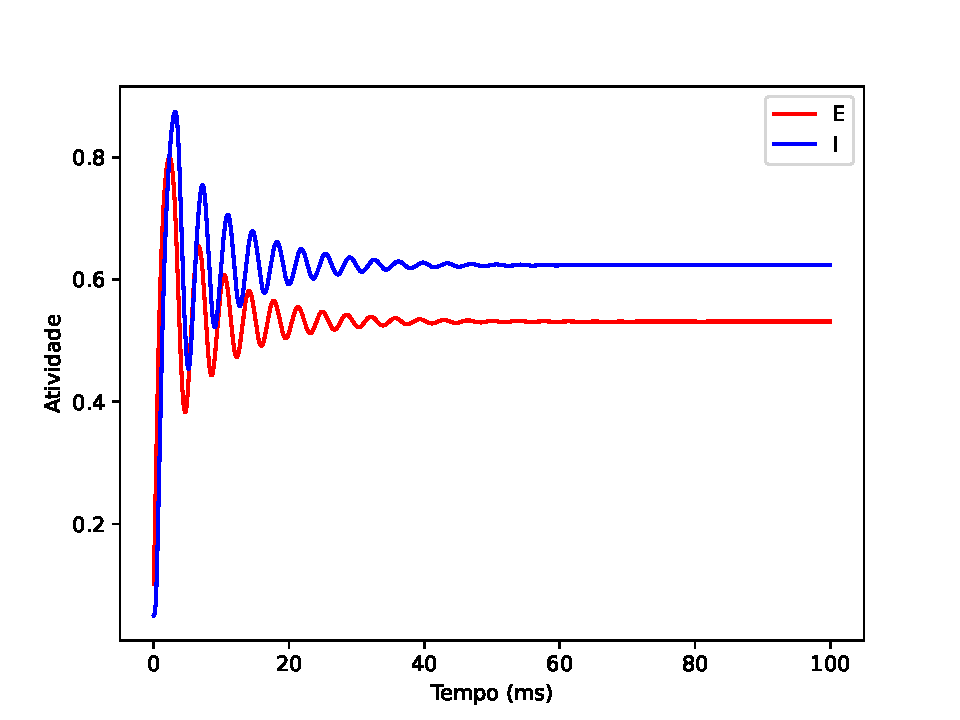
\includegraphics[width=\textwidth]{figs/ww_atividade}
		\end{subfigure}
		~
		\begin{subfigure}[b]{0.3\linewidth}
			\caption{Trajetória}
			\label{fig:ww_trajetoria}
			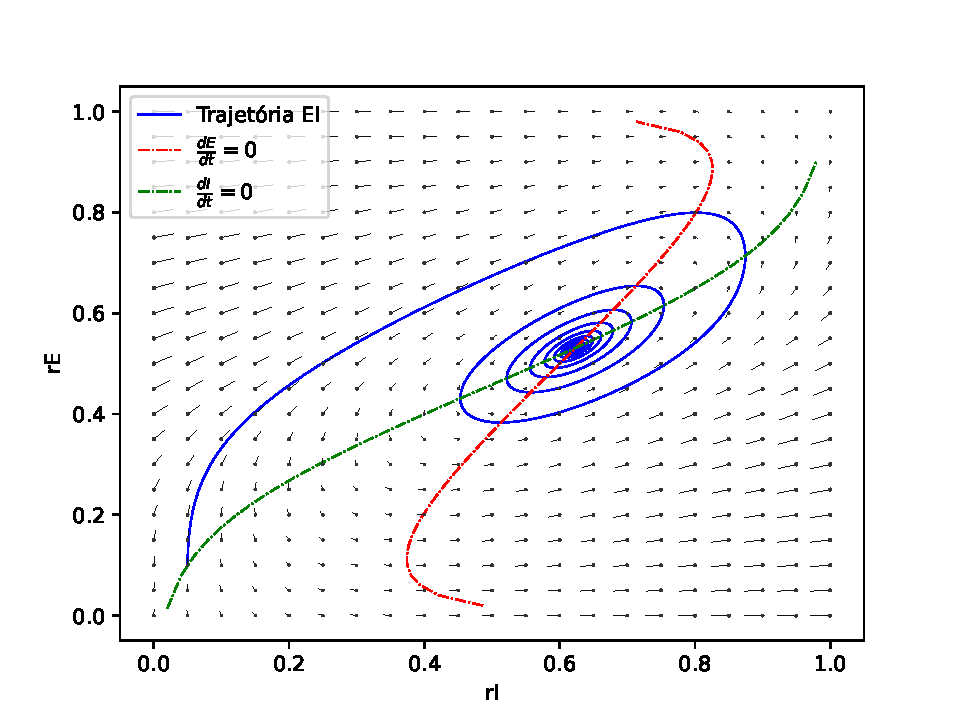
\includegraphics[width=\textwidth]{figs/ww_trajetoria}
		\end{subfigure}
%		\legend{Fonte: o autor (\the\year)}
	\end{figure}
	\[
		\tau_e\frac{\mathrm{d}r_e}{\mathrm{d}t} =-r_e+F_e(w_{ee}r_e-w_{ie}r_i+T_e(t))
		\quad
		\tau_i\frac{\mathrm{d}r_i}{\mathrm{d}t} =-r_i+F_i(w_{ei}r_e-w_{ii}r_i+T_i(t))
	\]
	\note{considera subpopulações excitatórias e inibitórias}
	\note{sistemas dinâmicos: se alteram ao longo do tempo (taxa de disparo)}
	\note{nullcline: trajetória quando as derivadas são nulas (taxa de disparo não se altera)}
\end{frame}

\subsection{Aprendizado e plasticidade de longa duração}
\begin{frame}{Plasticidade de longa duração}
	\begin{columns}[t]
		\column{5cm}
			\begin{figure}[tb]
				\centering
				\caption{Plasticidade dependente do tempo de disparo (STDP)}
				\label{fig:stdp}
				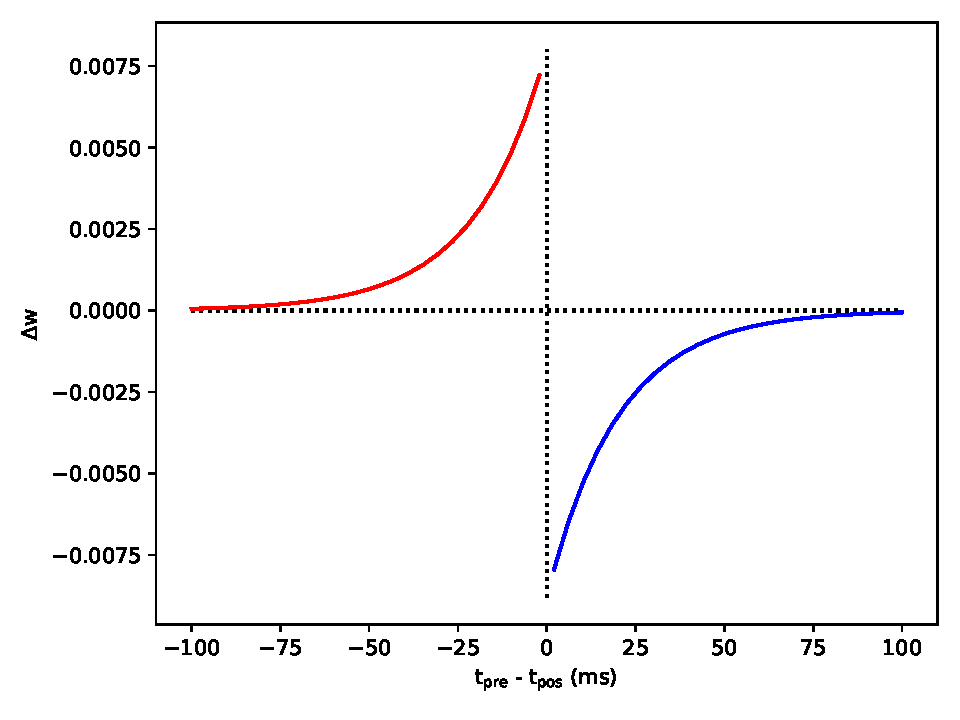
\includegraphics[width=\linewidth]{figs/stdp}
%				\legend{Fonte: o autor (\the\year)}
			\end{figure}
		\column{5cm}
			\begin{itemize}
				\note{Regra de Hebb: se um neurônio A excita um neurônio B repetidas vezes, então a sinapse entre os dois deve ser fortalecida}
				\item potencialização de longa duração: crescimento da força de conexão sináptica;
				\item depressão de longa duração: diminuição da força;
				\[
					\Delta_w=\begin{cases}
						A_+\exp(\Delta t/\tau_+)\text{, }\Delta t<0\\
						-A_-\exp(-\Delta t/\tau_-)\text{, }\Delta t\geq0
					\end{cases}
				\]
				\note{$A_+$ e $A_-$: valores máximos de modificação sináptica}
				\note{$\tau_+$ e $\tau_-$: faixas de intervalo entre disparo das células pré e pós-sinápticas}
			\end{itemize}
	\end{columns}
\end{frame}

	\section{Inteligência artificial}

\begin{frame}{Aprendizado de máquina}
	\begin{description}[aprendizado não-supervisionado]
		\item[Aprendizado supervisionado] utiliza pares de entrada-saída (rotulados) para aprender;
		\item[aprendizado não-supervisionado] tenta aprender padrões nos dados, como grupos de exemplos similares;
		\item[classificação] identifica a classe da informação;
		\note{exemplo classificação: identificar se um animal é cão ou gato\\}
		\item[agrupamento] determina classes agrupando informações similares em grupos (\textit{clusters})
		\note{exemplo agrupamento: agrupamento de filmes em gêneros\\}
		\item[regressão] prevê algum valor ou quantidade
		\note{exemplo regressão: prever o preço de ações ao longo do tempo\\}
		\item[redução de dimensionalidade] representa dados de várias dimensões em outras menores
		\note{exemplo redução de dimensionalidade: várias informações de um paciente sendo reduzidas às mais importantes para o diagnóstico de uma doença}
	\end{description}
\end{frame}

\subsection{Redes neurais}
\begin{frame}{Redes neurais}
	\begin{figure}
		\centering
		\caption{Arquiteturas do Perceptron}
		\label{fig:perceptrons}
		\begin{subfigure}[b]{0.3\textwidth}
			\caption{Perceptron}
			\label{fig:perceptron}
			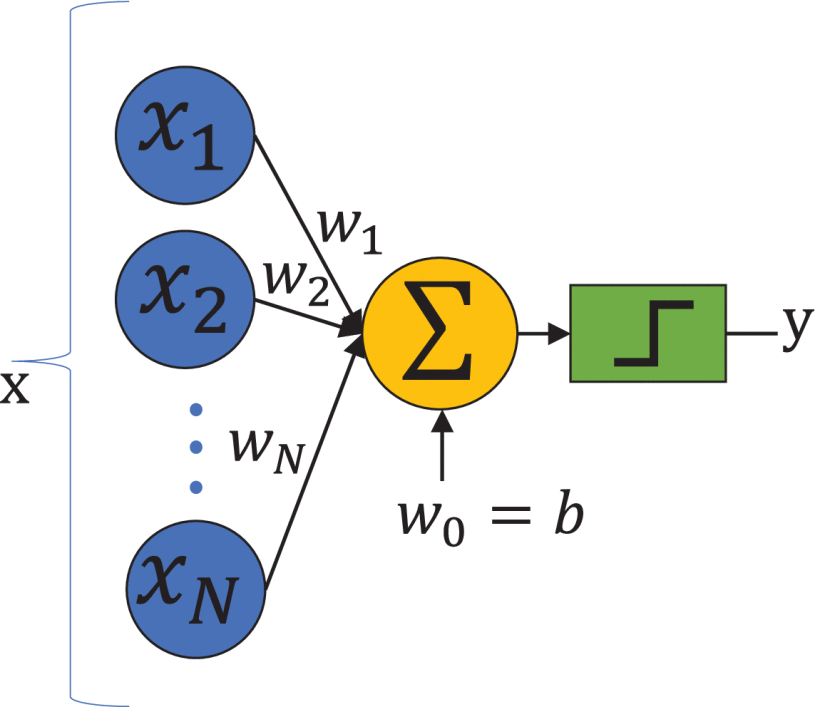
\includegraphics[width=\textwidth]{figs/perceptron}
		\end{subfigure}
		\qquad\qquad
		\begin{subfigure}[b]{0.3\textwidth}
			\caption{Perceptron de multi-camadas}
			\label{fig:mlp}
			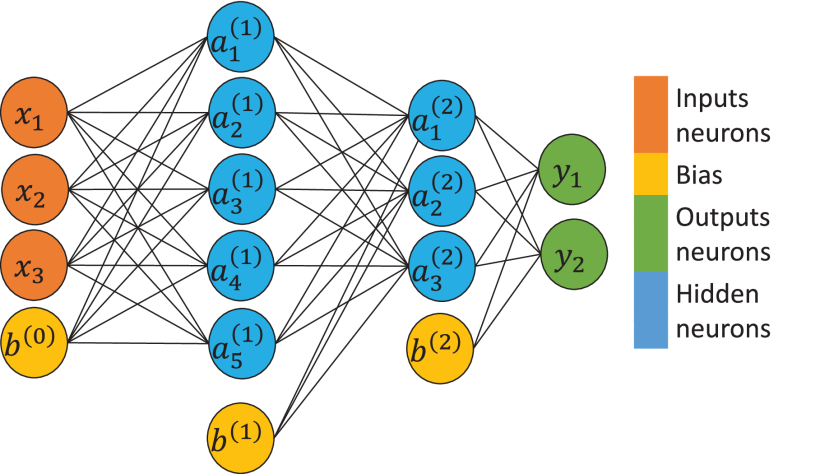
\includegraphics[width=\textwidth]{figs/mlp}
		\end{subfigure}
%		\fonte{\cite{parhi_brain-inspired_2020}}
	\end{figure}
	\note{perceptron: base do aprendizado de máquina\\}
	\note{$x_k$ é a resposta da sinapse $k$, $w_k$ é o peso da sinapse, $b$ é o \textit{bias} (viés, em português), um peso de referência que representa um conhecimento a priori, $\sigma$ é uma função de ativação não-linear, e $y$ é a saída do neurônio\\}
	\note{perceptron sozinho não é capaz de realizar tarefas de separação linear: MLP\\}
	\note{atualização dos pesos através do gradiente descendente (minimização do erro entre saída da rede e real)\\}
	\note{atualização com a metodologia da retropropagação: atualização das camadas finais em direção às iniciais\\}
	\note{quando a quantidade de camadas na rede é grande é chamada de rede neural profunda}
\end{frame}

\begin{frame}{Arquiteturas de redes neurais artificiais}
	\begin{itemize}
		\item \textit{Convolutional Neural Networks} (CNN, Redes neurais convolucionais)
		\note{CNN: possui camadas que implementam a operação matemática de convolução, aplicando um filtro no sinal, e camadas de sub-amostragem (\textit{downsampling}), chamadas de \textit{pooling}\\}
		\item \textit{Recurrent Neural Networks} (RNN, Redes neurais recorrentes)
		\note{RNN: possem a característica de processar os dados elemento a elemento, considerando também informações dos elementos passados, armazenados em pesos de conexões recorrentes, que funcionam como uma memória dinâmica para a rede\\}
		\item \textit{Hopfield Networks} (Redes Hopfield)
		\note{Hopfield: são redes treinadas para aprender padrões (memórias) dos dados de maneira associativa, baseado no princípio de Hebb \\}
		\item \textit{Autoencoder} (auto codificador)
		\note{autoencoder: redes que aprendem a representar os dados reduzindo sua dimensionalidade, diminuindo as camadas ocultas, e, posteriormente, recriando os dados originais\\}
		\item \textit{Long Short-Term Memory} (LSTM, memória longa de curto prazo)
		\note{LSTM: uma variação da RNN composta de 4~(quatro) blocos de memória, sendo um principal e os outros três, chamados de portões de entrada, esquecimento e saída, responsáveis por alterar o estado da célula como um todo}
	\end{itemize}
\end{frame}

\subsection{Redes neuromórficas}
\begin{frame}{Redes neuromórficas}
	\begin{columns}[t]
		\column{5cm}
			\begin{figure}[tb]
				\centering
				\caption{Arquitetura de redes neurais de disparo (SNN)}
				\label{fig:snn}
				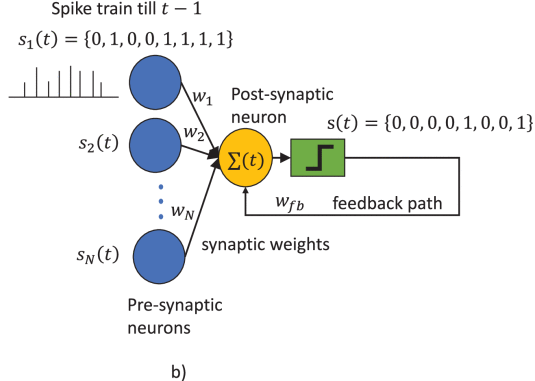
\includegraphics[width=\linewidth]{figs/snn}
%				\fonte{\cite{parhi_brain-inspired_2020}}
			\end{figure}
		\column{5cm}
			\begin{itemize}
				\item Distribui o processamento e memória em conjunto nos elementos de neurônio e sinapse;
				\note{von neumann: memória e processamento ficam separadas\\}
				\item informação codificada em sequências de potenciais de ação;
				\note{von neumann: codificação para sinais binários (0 e 1)\\}
				\item programas definidos pela estrutura da rede neural e seus parâmetros.
				\note{von neumann: programas escritos em instruções explícitas}
			\end{itemize}
	\end{columns}
\end{frame}

\begin{frame}{Redes neuromórficas}
	\begin{itemize}
		\item Usam, principalmente, neurônios do tipo integra-e-dispara;
		\item redes neurais convencionais podem ser convertidas em redes de disparo fazendo ajustes de pesos e normalizações;
		\item dados de entrada precisam ser codificados em disparos de potencial de ação;
		\note{codificações baseadas em taxa de disparo, ordem dos disparos ou temporalmente\\}
		\item o aprendizado frequentemente usa a STDP para o não-supervisionado, e uma versão do \textit{backpropagation} para o supervisionado, relacionando ativações das unidades de redes neurais com taxas de disparo.
		\note{há discussões sobre o treinamento com backprop na simulação do cérebro}\\
		\note{57 min}
	\end{itemize}
\end{frame}

	\section{Considerações finais}
\begin{frame}{Considerações finais}
	\begin{columns}[t]
		\column{5cm}
			\begin{figure}[tb]
				\centering
				\caption{Ambiente do Google Colaboratory com o conteúdo de neurônios de disparo}
				\label{fig:colab}
				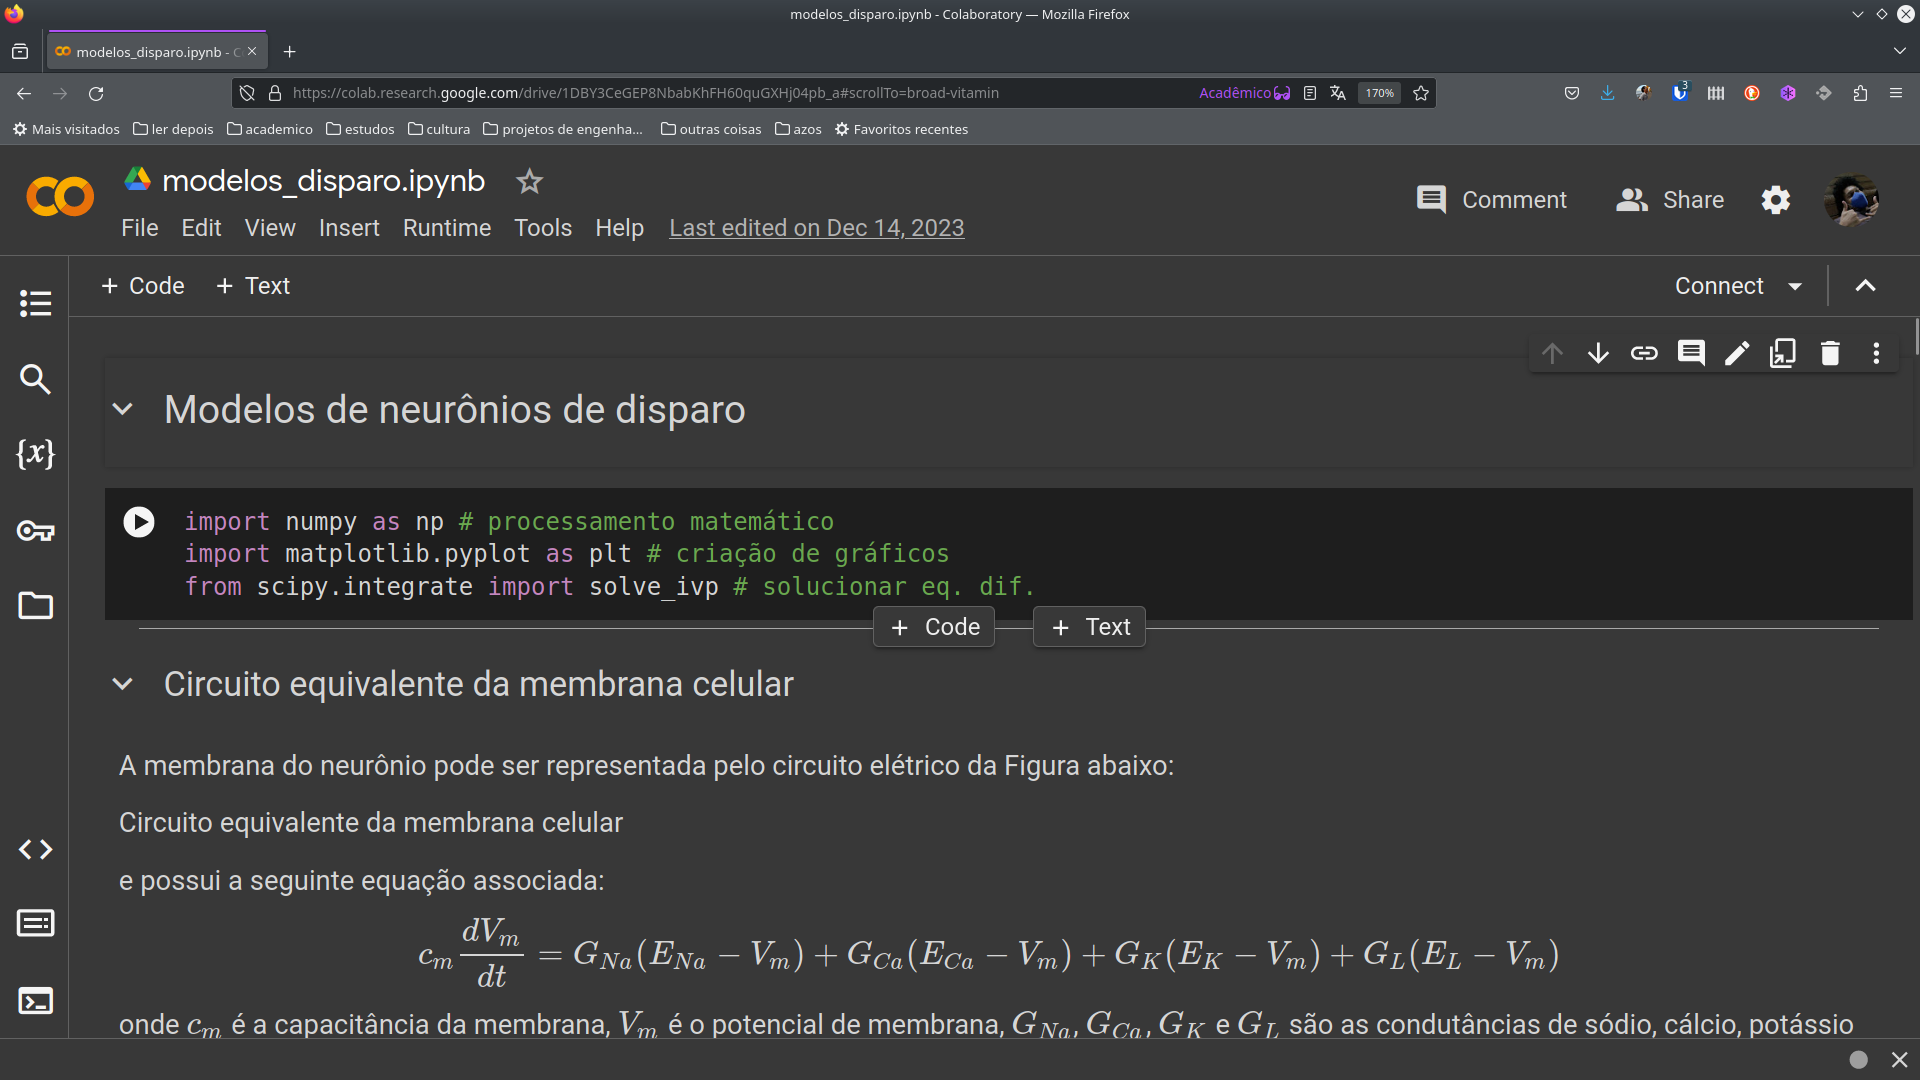
\includegraphics[width=\linewidth]{figs/colab}
%				\legend{Fonte: o autor (\the\year)}
			\end{figure}
		\column{5cm}
			\begin{itemize}
				\item Proposta de sequência didática gerada;
				\note{sequencia didatica: incluindo atividades avaliativas}
				\item códigos fontes em repositório online;
				\note{codigos fonte: incluindo os que geram algumas figuras do texto}
				\item novos conteúdos podem incluir a estimulação elétrica axonal, a análise de sinais de eletroencefalograma (EEG) e a apresentação de pacotes voltados à simulação neuronal.
				\note{estimulação elétrica: estudar a propagação do potencial de ação ao longo do axônio}
				\note{eeg: respostas elétricas obtidas das atividades cerebrais. podem ser utilizadas para associações com comorbidades, como depressão e ansiedade}
				\note{pacotes: tem seu entendimento facilitado pós conteúdo deste curso}
			\end{itemize}
	\end{columns}
\end{frame}


	%%------------------------------------------------
	%\section*{Referências}
	%%------------------------------------------------
	%\begin{frame}[noframenumbering]
	\begin{frame}
		\frametitle{Referências}
		\footnotesize{
			\begin{thebibliography}{99} % Beamer does not support BibTeX so references must be inserted manually as below
				\bibitem[DAYAN, P.; ABBOTT, L. F; 2001]{p1} Peter Dayan, F. F. Abbott (2001)
				\newblock Theoretical neuroscience: computational and mathematical modeling of neural systems
				\newblock \emph{Computational Neuroscience}, Massachusetts Institute of Tecnology Press.
				
				\bibitem[ERMENTROUT; 2010]{p2} Bard Ermentrout, David Terman (2010)
				\newblock Mathematical foundations of neuroscience
				\newblock \emph{Interdisciplinary applied mathematics}, Springer.
				
				\bibitem[Miller, Paul; 2018]{p3} 
				Paul Miller (2018)
				\newblock An Introductory Course in Computational Neuroscience
				\newblock \emph{Computational Neuroscience}, Massachusetts Institute of Tecnology Press.
			\end{thebibliography}
		}
	\end{frame}

	\section*{}
	\begin{frame}[noframenumbering]
	\centering
	\textbf{Muito obrigado!}
	\end{frame}

\end{document} 
